In this section, we describe the results of the three experiments mentioned earlier.

\subsection{Multitenancy and elasticity experiment}
In Figure~\ref{fig:multitenancyexp}, it can clearly be seen that multiple jobs can be accepted simultaneously by the system.
Also, we can see the number of running worker nodes increase and decrease with demand.
At 200 seconds, we see that the maximum number of worker nodes has been reached, and we no longer have three worker nodes per job.

\begin{figure}[ht!]
    \center
    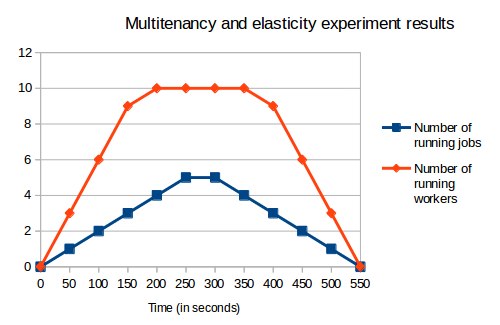
\includegraphics[width=0.45\textwidth]{./img/multitenancyexp.png}
    \caption{Results of the Multitenancy and elasticity experiment}
    \label{fig:multitenancyexp}
\end{figure}

Every 50 seconds of the first 300 seconds, a job was added by a user.
Most jobs took about 200 seconds.


\subsection{Load balancing experiment}
As can be seen in Figure~\ref{fig:loadbalancingexp}, the time spent processing by the worker nodes is rather balanced.
This means that splitting a job of rendering a movie into tasks of rendering a frame is enough to efficiently divide the work over multiple nodes.

\begin{figure}[ht!]
    \center
    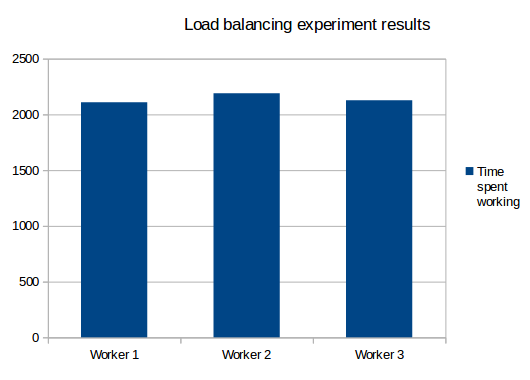
\includegraphics[width=0.45\textwidth]{./img/loadbalancingexp.png}
    \caption{Results of the Load balancing experiment}
    \label{fig:loadbalancingexp}
\end{figure}

\subsection{Reliability experiment}
Of the 25 tasks that were interrupted by killing off a worker, all 25 of them were restarted by the master node and finished by some other worker.
This experiment by no means proves that tasks cannot be lost.
However, it does show some robustness against workers losing their connection with the master node somehow.

\subsection{Cost analysis}
The largest movie, or job, rendered on the DAS-4 server was a movie of 300 frames and ten seconds long.
It had 1000 samples per pixel and a resolution of ($800 \times 600$).
DAS-4 was configured with one master node and ten worker nodes.
The total computation  time to render the movie was ten hours.
In total this is 11 machines $\times$ 10 hours $=$ 110 instance hours.
Assuming that an Amazon EC2 instance is as fast as a DAS-4 instance and that an Amazon EC2 instance is charged for \EUR$0,10$ per instance hour, rendering the ten seconds movie would cost \EUR{$11,00$}, which is \EUR$1,10$ to render one second of a movie.

If rendering is not going to be a core business, it is advised to make use of the Amazon Web Services.
Investing in dedicated hardware is not recommended, since it would be too expensive to be worth it.

However, if rendering is core business, then it is advisable to purchase dedicated hardware.
\EUR$1,10$ per second of a movie is quite expensive, especially if a lot of movies are going to be rendered.
For core business rendering, purchasing dedicated hardware could definitely save money.